\section{Pensando como economista}
\subsection{Modelos económicos}
Los economista utilizan modelos creados bajo ciertos supuestos para simplificar la realidad con el fin de mejorar nuestra comprensión del mundo. Dos de los modelos económicos más básicos son:
\begin{itemize}
	\item El diagrama de flujo circular: explicar en términos generales cómo se organiza la economía y la manera en que los diferentes acotres interactúan
	\item La frontera de posibilidades de producción: la herramienta matemática más simple en economía
\end{itemize}

\begingroup
\setlength{\tabcolsep}{5pt} % Default value: 6pt
\renewcommand{\arraystretch}{1.5} % Default value: 1
\begin{center}
	\begin{tabular}{p{3.5cm}|p{13cm}}
		Modelo&Explicacion\\ \hline
		Diagrama de flujo circular&El {\bf diagrama de flujo circular} es un modelo visual de la economía que muestra cómo el dinero fluyen a través de los mercados entre los hogares y las empresas.\\
		Frontera de posibilidades de producción& La {\bf frontera de posibilidades de producción} es un gráfico que muestra las combinaciones de producción que la economía puede generar dados los factores de producción y la tecnología disponible
	\end{tabular}
\end{center}
\endgroup
\begingroup
\setlength{\tabcolsep}{5pt} % Default value: 6pt
\renewcommand{\arraystretch}{1.5} % Default value: 1
\begin{center}
	\begin{figure}[h]
		\centering
\begin{subfigure}	
	\left
	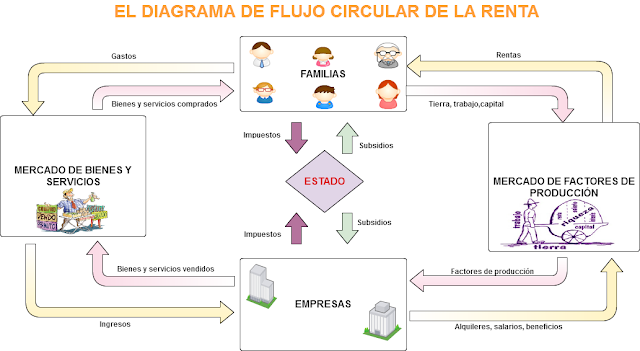
\includegraphics[scale=0.3]{images/FlujoCircular.png}
\end{subfigure} 	
\begin{subfigure}
	\left	
	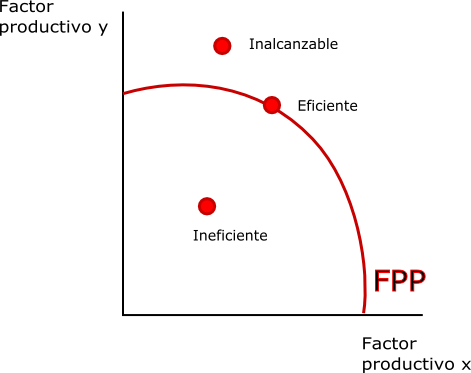
\includegraphics[scale=0.3]{images/FPP.png}
\end{subfigure} 		
	\end{figure}
\end{center}

\endgroup
\begingroup
\setlength{\tabcolsep}{5pt} % Default value: 6pt
\renewcommand{\arraystretch}{1.5} % Default value: 1
\begin{center}
	\begin{tabular}{l|l}
		{\bf Microeconomía}&Se centra en las partes individuales de la economía.\\ \hline
		{\bf Macroeconomía}&Mira a la economía en su conjunto
	\end{tabular}
\end{center}
\endgroup

\subsection{Los economistas como asesores políticos}
Cuando los economistas tratan de explicar como es el mundo se les puede tratar como \underline{científicos}. Sin embargo, cuando un economista intenta darle forma al mundo, son \underline{asesores políticos}. Debido a lo anterior ambos usan el lenguaje de manera distinta. Para eso existen diferentes tipos de afirmaciones:

\begingroup
\setlength{\tabcolsep}{5pt} % Default value: 6pt
\renewcommand{\arraystretch}{1.5} % Default value: 1
\begin{center}
\begin{tabular}{p{1.7cm}|p{11cm}}
{\bf Positiva}& Es descriptiva y se refiere a cómo es el mundo. Esta se tiende a usar más cuando el area es mas cientifica\\ \hline
{\bf Normativa}& Es prescriptiva y se refiere a cómo deberia de ser el mundo. Esta se tiende a usar más cuando buscamo políticas que son deseables
\end{tabular}
\end{center}
\endgroup

Debido a que todos utilizamos el lenguaje de manera distinta, los economistas tienden a discrepar entre sí. Estas discrepancias se pueden causar por no estar de acuerdo con la validez de otras teorías positivas, pero tambien se pueden causar porque cada economista puede tener sus propios valores. Y con ello teber distintas viciones normativas de lo que la política económica devería tratar de lograr.
